
%% bare_conf.tex
%% V1.3
%% 2007/01/11
%% by Michael Shell
%% See:
%% http://www.michaelshell.org/
%% for current contact information.
%%
%% This is a skeleton file demonstrating the use of IEEEtran.cls
%% (requires IEEEtran.cls version 1.7 or later) with an IEEE conference paper.
%%
%% Support sites:
%% http://www.michaelshell.org/tex/ieeetran/
%% http://www.ctan.org/tex-archive/macros/latex/contrib/IEEEtran/
%% and
%% http://www.ieee.org/

%%*************************************************************************
%% Legal Notice:
%% This code is offered as-is without any warranty either expressed or
%% implied; without even the implied warranty of MERCHANTABILITY or
%% FITNESS FOR A PARTICULAR PURPOSE!
%% User assumes all risk.
%% In no event shall IEEE or any contributor to this code be liable for
%% any damages or losses, including, but not limited to, incidental,
%% consequential, or any other damages, resulting from the use or misuse
%% of any information contained here.
%%
%% All comments are the opinions of their respective authors and are not
%% necessarily endorsed by the IEEE.
%%
%% This work is distributed under the LaTeX Project Public License (LPPL)
%% ( http://www.latex-project.org/ ) version 1.3, and may be freely used,
%% distributed and modified. A copy of the LPPL, version 1.3, is included
%% in the base LaTeX documentation of all distributions of LaTeX released
%% 2003/12/01 or later.
%% Retain all contribution notices and credits.
%% ** Modified files should be clearly indicated as such, including  **
%% ** renaming them and changing author support contact information. **
%%
%% File list of work: IEEEtran.cls, IEEEtran_HOWTO.pdf, bare_adv.tex,
%%                    bare_conf.tex, bare_jrnl.tex, bare_jrnl_compsoc.tex
%%*************************************************************************

% *** Authors should verify (and, if needed, correct) their LaTeX system  ***
% *** with the testflow diagnostic prior to trusting their LaTeX platform ***
% *** with production work. IEEE's font choices can trigger bugs that do  ***
% *** not appear when using other class files.                            ***
% The testflow support page is at:
% http://www.michaelshell.org/tex/testflow/



% Note that the a4paper option is mainly intended so that authors in
% countries using A4 can easily print to A4 and see how their papers will
% look in print - the typesetting of the document will not typically be
% affected with changes in paper size (but the bottom and side margins will).
% Use the testflow package mentioned above to verify correct handling of
% both paper sizes by the user's LaTeX system.
%
% Also note that the "draftcls" or "draftclsnofoot", not "draft", option
% should be used if it is desired that the figures are to be displayed in
% draft mode.
%
\documentclass[conference]{IEEEtran}
% Add the compsoc option for Computer Society conferences.
%
% If IEEEtran.cls has not been installed into the LaTeX system files,
% manually specify the path to it like:
% \documentclass[conference]{../sty/IEEEtran}


\makeatletter
\def\ps@headings{%
\def\@oddhead{\mbox{}\scriptsize\rightmark \hfil \thepage}%
\def\@evenhead{\scriptsize\thepage \hfil \leftmark\mbox{}}%
\def\@oddfoot{}%
\def\@evenfoot{}}
\makeatother

\pagestyle{headings}
\usepackage{amsfonts}
\usepackage{amsthm}
\usepackage{amssymb}
\usepackage{amsmath}
\usepackage{graphicx}
\usepackage{fancyhdr}

\newtheorem{Prop}{Proposition}
\newtheorem{lemma}{Lemma}
\newtheorem{theorem}{Theorem}


% Some very useful LaTeX packages include:
% (uncomment the ones you want to load)


% *** MISC UTILITY PACKAGES ***
%
%\usepackage{ifpdf}
% Heiko Oberdiek's ifpdf.sty is very useful if you need conditional
% compilation based on whether the output is pdf or dvi.
% usage:
% \ifpdf
%   % pdf code
% \else
%   % dvi code
% \fi
% The latest version of ifpdf.sty can be obtained from:
% http://www.ctan.org/tex-archive/macros/latex/contrib/oberdiek/
% Also, note that IEEEtran.cls V1.7 and later provides a builtin
% \ifCLASSINFOpdf conditional that works the same way.
% When switching from latex to pdflatex and vice-versa, the compiler may
% have to be run twice to clear warning/error messages.






% *** CITATION PACKAGES ***
%
%\usepackage{cite}
% cite.sty was written by Donald Arseneau
% V1.6 and later of IEEEtran pre-defines the format of the cite.sty package
% \cite{} output to follow that of IEEE. Loading the cite package will
% result in citation numbers being automatically sorted and properly
% "compressed/ranged". e.g., [1], [9], [2], [7], [5], [6] without using
% cite.sty will become [1], [2], [5]--[7], [9] using cite.sty. cite.sty's
% \cite will automatically add leading space, if needed. Use cite.sty's
% noadjust option (cite.sty V3.8 and later) if you want to turn this off.
% cite.sty is already installed on most LaTeX systems. Be sure and use
% version 4.0 (2003-05-27) and later if using hyperref.sty. cite.sty does
% not currently provide for hyperlinked citations.
% The latest version can be obtained at:
% http://www.ctan.org/tex-archive/macros/latex/contrib/cite/
% The documentation is contained in the cite.sty file itself.






% *** GRAPHICS RELATED PACKAGES ***
%
\ifCLASSINFOpdf
  % \usepackage[pdftex]{graphicx}
  % declare the path(s) where your graphic files are
  % \graphicspath{{../pdf/}{../jpeg/}}
  % and their extensions so you won't have to specify these with
  % every instance of \includegraphics
  % \DeclareGraphicsExtensions{.pdf,.jpeg,.png}
\else
  % or other class option (dvipsone, dvipdf, if not using dvips). graphicx
  % will default to the driver specified in the system graphics.cfg if no
  % driver is specified.
  % \usepackage[dvips]{graphicx}
  % declare the path(s) where your graphic files are
  % \graphicspath{{../eps/}}
  % and their extensions so you won't have to specify these with
  % every instance of \includegraphics
  % \DeclareGraphicsExtensions{.eps}
\fi
% graphicx was written by David Carlisle and Sebastian Rahtz. It is
% required if you want graphics, photos, etc. graphicx.sty is already
% installed on most LaTeX systems. The latest version and documentation can
% be obtained at:
% http://www.ctan.org/tex-archive/macros/latex/required/graphics/
% Another good source of documentation is "Using Imported Graphics in
% LaTeX2e" by Keith Reckdahl which can be found as epslatex.ps or
% epslatex.pdf at: http://www.ctan.org/tex-archive/info/
%
% latex, and pdflatex in dvi mode, support graphics in encapsulated
% postscript (.eps) format. pdflatex in pdf mode supports graphics
% in .pdf, .jpeg, .png and .mps (metapost) formats. Users should ensure
% that all non-photo figures use a vector format (.eps, .pdf, .mps) and
% not a bitmapped formats (.jpeg, .png). IEEE frowns on bitmapped formats
% which can result in "jaggedy"/blurry rendering of lines and letters as
% well as large increases in file sizes.
%
% You can find documentation about the pdfTeX application at:
% http://www.tug.org/applications/pdftex





% *** MATH PACKAGES ***
%
%\usepackage[cmex10]{amsmath}
% A popular package from the American Mathematical Society that provides
% many useful and powerful commands for dealing with mathematics. If using
% it, be sure to load this package with the cmex10 option to ensure that
% only type 1 fonts will utilized at all point sizes. Without this option,
% it is possible that some math symbols, particularly those within
% footnotes, will be rendered in bitmap form which will result in a
% document that can not be IEEE Xplore compliant!
%
% Also, note that the amsmath package sets \interdisplaylinepenalty to 10000
% thus preventing page breaks from occurring within multiline equations. Use:
%\interdisplaylinepenalty=2500
% after loading amsmath to restore such page breaks as IEEEtran.cls normally
% does. amsmath.sty is already installed on most LaTeX systems. The latest
% version and documentation can be obtained at:
% http://www.ctan.org/tex-archive/macros/latex/required/amslatex/math/





% *** SPECIALIZED LIST PACKAGES ***
%
%\usepackage{algorithmic}
% algorithmic.sty was written by Peter Williams and Rogerio Brito.
% This package provides an algorithmic environment fo describing algorithms.
% You can use the algorithmic environment in-text or within a figure
% environment to provide for a floating algorithm. Do NOT use the algorithm
% floating environment provided by algorithm.sty (by the same authors) or
% algorithm2e.sty (by Christophe Fiorio) as IEEE does not use dedicated
% algorithm float types and packages that provide these will not provide
% correct IEEE style captions. The latest version and documentation of
% algorithmic.sty can be obtained at:
% http://www.ctan.org/tex-archive/macros/latex/contrib/algorithms/
% There is also a support site at:
% http://algorithms.berlios.de/index.html
% Also of interest may be the (relatively newer and more customizable)
% algorithmicx.sty package by Szasz Janos:
% http://www.ctan.org/tex-archive/macros/latex/contrib/algorithmicx/




% *** ALIGNMENT PACKAGES ***
%
%\usepackage{array}
% Frank Mittelbach's and David Carlisle's array.sty patches and improves
% the standard LaTeX2e array and tabular environments to provide better
% appearance and additional user controls. As the default LaTeX2e table
% generation code is lacking to the point of almost being broken with
% respect to the quality of the end results, all users are strongly
% advised to use an enhanced (at the very least that provided by array.sty)
% set of table tools. array.sty is already installed on most systems. The
% latest version and documentation can be obtained at:
% http://www.ctan.org/tex-archive/macros/latex/required/tools/


%\usepackage{mdwmath}
%\usepackage{mdwtab}
% Also highly recommended is Mark Wooding's extremely powerful MDW tools,
% especially mdwmath.sty and mdwtab.sty which are used to format equations
% and tables, respectively. The MDWtools set is already installed on most
% LaTeX systems. The lastest version and documentation is available at:
% http://www.ctan.org/tex-archive/macros/latex/contrib/mdwtools/


% IEEEtran contains the IEEEeqnarray family of commands that can be used to
% generate multiline equations as well as matrices, tables, etc., of high
% quality.


%\usepackage{eqparbox}
% Also of notable interest is Scott Pakin's eqparbox package for creating
% (automatically sized) equal width boxes - aka "natural width parboxes".
% Available at:
% http://www.ctan.org/tex-archive/macros/latex/contrib/eqparbox/





% *** SUBFIGURE PACKAGES ***
%\usepackage[tight,footnotesize]{subfigure}
% subfigure.sty was written by Steven Douglas Cochran. This package makes it
% easy to put subfigures in your figures. e.g., "Figure 1a and 1b". For IEEE
% work, it is a good idea to load it with the tight package option to reduce
% the amount of white space around the subfigures. subfigure.sty is already
% installed on most LaTeX systems. The latest version and documentation can
% be obtained at:
% http://www.ctan.org/tex-archive/obsolete/macros/latex/contrib/subfigure/
% subfigure.sty has been superceeded by subfig.sty.



%\usepackage[caption=false]{caption}
%\usepackage[font=footnotesize]{subfig}
% subfig.sty, also written by Steven Douglas Cochran, is the modern
% replacement for subfigure.sty. However, subfig.sty requires and
% automatically loads Axel Sommerfeldt's caption.sty which will override
% IEEEtran.cls handling of captions and this will result in nonIEEE style
% figure/table captions. To prevent this problem, be sure and preload
% caption.sty with its "caption=false" package option. This is will preserve
% IEEEtran.cls handing of captions. Version 1.3 (2005/06/28) and later
% (recommended due to many improvements over 1.2) of subfig.sty supports
% the caption=false option directly:
%\usepackage[caption=false,font=footnotesize]{subfig}
%
% The latest version and documentation can be obtained at:
% http://www.ctan.org/tex-archive/macros/latex/contrib/subfig/
% The latest version and documentation of caption.sty can be obtained at:
% http://www.ctan.org/tex-archive/macros/latex/contrib/caption/




% *** FLOAT PACKAGES ***
%
%\usepackage{fixltx2e}
% fixltx2e, the successor to the earlier fix2col.sty, was written by
% Frank Mittelbach and David Carlisle. This package corrects a few problems
% in the LaTeX2e kernel, the most notable of which is that in current
% LaTeX2e releases, the ordering of single and double column floats is not
% guaranteed to be preserved. Thus, an unpatched LaTeX2e can allow a
% single column figure to be placed prior to an earlier double column
% figure. The latest version and documentation can be found at:
% http://www.ctan.org/tex-archive/macros/latex/base/



%\usepackage{stfloats}
% stfloats.sty was written by Sigitas Tolusis. This package gives LaTeX2e
% the ability to do double column floats at the bottom of the page as well
% as the top. (e.g., "\begin{figure*}[!b]" is not normally possible in
% LaTeX2e). It also provides a command:
%\fnbelowfloat
% to enable the placement of footnotes below bottom floats (the standard
% LaTeX2e kernel puts them above bottom floats). This is an invasive package
% which rewrites many portions of the LaTeX2e float routines. It may not work
% with other packages that modify the LaTeX2e float routines. The latest
% version and documentation can be obtained at:
% http://www.ctan.org/tex-archive/macros/latex/contrib/sttools/
% Documentation is contained in the stfloats.sty comments as well as in the
% presfull.pdf file. Do not use the stfloats baselinefloat ability as IEEE
% does not allow \baselineskip to stretch. Authors submitting work to the
% IEEE should note that IEEE rarely uses double column equations and
% that authors should try to avoid such use. Do not be tempted to use the
% cuted.sty or midfloat.sty packages (also by Sigitas Tolusis) as IEEE does
% not format its papers in such ways.





% *** PDF, URL AND HYPERLINK PACKAGES ***
%
%\usepackage{url}
% url.sty was written by Donald Arseneau. It provides better support for
% handling and breaking URLs. url.sty is already installed on most LaTeX
% systems. The latest version can be obtained at:
% http://www.ctan.org/tex-archive/macros/latex/contrib/misc/
% Read the url.sty source comments for usage information. Basically,
% \url{my_url_here}.





% *** Do not adjust lengths that control margins, column widths, etc. ***
% *** Do not use packages that alter fonts (such as pslatex).         ***
% There should be no need to do such things with IEEEtran.cls V1.6 and later.
% (Unless specifically asked to do so by the journal or conference you plan
% to submit to, of course. )


% correct bad hyphenation here
% \hyphenation{op-tical net-works semi-conduc-tor}


\newcommand{\br}{{\mathbf r}}
\newcommand{\bA}{{\mathbf A}}
\newcommand{\ba}{{\bf a}}
\newcommand{\bb}{{\bf b}}
\newcommand{\bc}{{\bf c}}
\newcommand{\bC}{{\bf C}}
\newcommand{\bd}{{\bf d}}
\newcommand{\be}{{\bf e}}
\newcommand{\bE}{{\bf E}}
\newcommand{\bbf}{{\bf f}}
\newcommand{\bF}{{\bf F}}
\newcommand{\bh}{{\bf h}}
\newcommand{\bH}{{\bf H}}
\newcommand{\bg}{{\bf g}}
\newcommand{\bG}{{\bf G}}
\newcommand{\bq}{{\bf q}}
\newcommand{\bs}{{\bf s}}
\newcommand{\bm}{{\bf m}}
\newcommand{\bn}{{\bf n}}
\newcommand{\bu}{{\bf u}}
\newcommand{\bv}{{\bf v}}
\newcommand{\bw}{{\bf w}}
\newcommand{\bx}{{\bf x}}
\newcommand{\by}{{\bf y}}
\newcommand{\bz}{{\bf z}}
\newcommand{\bL}{{\bf L}}
\newcommand{\bM}{{\bf M}}
\newcommand{\bN}{{\bf N}}
\newcommand{\bS}{{\bf S}}
\newcommand{\bT}{{\bf T}}
\newcommand{\bD}{{\bf D}}
\newcommand{\bX}{{\bf X}}
\newcommand{\bP}{{\bf P}}
\newcommand{\bQ}{{\bf Q}}
\newcommand{\bI}{{\bf I}}
\newcommand{\bR}{{\bf R}}
\newcommand{\bU}{{\bf U}}
\newcommand{\bV}{{\bf V}}
\newcommand{\bW}{{\bf W}}
\newcommand{\bY}{{\bf Y}}
\newcommand{\bZ}{{\bf Z}}
\newcommand{\bJ}{{\bf J}}
\newcommand{\bB}{{\bf B}}
\newcommand{\bzero}{{\bf 0}}
\newcommand{\bgamma}{{\mbox {\boldmath $\gamma$}}}
\newcommand{\btheta}{{\mbox {\boldmath $\theta$}}}
\newcommand{\bvartheta}{{\mbox {\boldmath $\vartheta$}}}
\newcommand{\bDelta}{{\mbox {\boldmath $\Delta$}}}
\newcommand{\bLambda}{{\mbox {\boldmath $\Lambda$}}}
\newcommand{\bPsi}{{\mbox {\boldmath $\Psi$}}}
\newcommand{\bPhi}{{\mbox {\boldmath $\Phi$}}}
\newcommand{\bcA}{{\mbox {\boldmath ${\cal A}$}}}
\newcommand{\bcB}{{\mbox {\boldmath ${\cal B}$}}}
\newcommand{\bcC}{{\mbox {\boldmath ${\cal C}$}}}
\newcommand{\bcD}{{\mbox {\boldmath ${\cal D}$}}}
\newcommand{\bcF}{{\mbox {\boldmath ${\cal F}$}}}
\newcommand{\bcG}{{\mbox {\boldmath ${\cal G}$}}}
\newcommand{\bcL}{{\mbox {\boldmath ${\cal L}$}}}
\newcommand{\bcN}{{\mbox {\boldmath ${\cal N}$}}}
\newcommand{\bcR}{{\mbox {\boldmath ${\cal R}$}}}
\newcommand{\bcS}{{\mbox {\boldmath ${\cal S}$}}}
\newcommand{\bcH}{{\mbox {\boldmath ${\cal H}$}}}
\newcommand{\bcI}{{\mbox {\boldmath ${\cal I}$}}}
\newcommand{\bcO}{{\mbox {\boldmath ${\cal O}$}}}
\newcommand{\bcP}{{\mbox {\boldmath ${\cal P}$}}}
\newcommand{\bcQ}{{\mbox {\boldmath ${\cal Q}$}}}
\newcommand{\bcV}{{\mbox {\boldmath ${\cal V}$}}}
\newcommand{\bcW}{{\mbox {\boldmath ${\cal W}$}}}


\begin{document}
%
% paper title
% can use linebreaks \\ within to get better formatting as desired
\title{Optimizing Enhanced Hierarchical Modulations}


% author names and affiliations
% use a multiple column layout for up to three different
% affiliations
\author{\IEEEauthorblockN{Shu Wang, Jungwon Min and Byung K. Yi}
%\author{%\IEEEauthorblockN{Diet Koffee}
\IEEEauthorblockA{LG Electronics Mobile Research\\
San Diego, CA 92131-1639
% Email: \{swang,\ jungwonmin,\ byungkyi\}@lge.com} }
} }

% conference papers do not typically use \thanks and this command
% is locked out in conference mode. If really needed, such as for
% the acknowledgment of grants, issue a \IEEEoverridecommandlockouts
% after \documentclass

% for over three affiliations, or if they all won't fit within the width
% of the page, use this alternative format:
%
%\author{\IEEEauthorblockN{Michael Shell\IEEEauthorrefmark{1},
%Homer Simpson\IEEEauthorrefmark{2},
%James Kirk\IEEEauthorrefmark{3},
%Montgomery Scott\IEEEauthorrefmark{3} and
%Eldon Tyrell\IEEEauthorrefmark{4}}
%\IEEEauthorblockA{\IEEEauthorrefmark{1}School of Electrical and Computer Engineering\\
%Georgia Institute of Technology,
%Atlanta, Georgia 30332--0250\\ Email: see http://www.michaelshell.org/contact.html}
%\IEEEauthorblockA{\IEEEauthorrefmark{2}Twentieth Century Fox, Springfield, USA\\
%Email: homer@thesimpsons.com}
%\IEEEauthorblockA{\IEEEauthorrefmark{3}Starfleet Academy, San Francisco, California 96678-2391\\
%Telephone: (800) 555--1212, Fax: (888) 555--1212}
%\IEEEauthorblockA{\IEEEauthorrefmark{4}Tyrell Inc., 123 Replicant Street, Los Angeles, California 90210--4321}}

% use for special paper notices
%\IEEEspecialpapernotice{(Invited Paper)}

% make the title area

\maketitle
\begin{abstract}\small
Hierarchical modulation offers an important coverage and
throughput tradeoff for wireless communications, but it has
received relatively little attention to date. Traditional
hierarchical modulation suffers from the interference between
layers, which results in both capacity loss and bit-error rate
increasing. In this paper, an enhanced hierarchical modulation
technique along with four optimization criteria are presented and
discussed. The proposed hierarchical modulation enhancement, where
the enhancement-layer signal constellation is carefully rotated,
can help achieve better performance with minimum complexity
increase. The first criterion is proposed to maximize the
achievable spectral efficiency with changing the Euclidean
distance profile. The second criterion is to lower demodulation
error rate with maximizing the modulation efficiency, which is the
concept suggested for quantizing the effect of inter-layer
interference. The third criterion is proposed to maximize the
demodulation robustness when the imperfect channel estimation
happened. The demodulation robustness is defined as the ratio
between the demodulation error and channel estimation error. The
last approach is suggested for maximizing the RF power amplifier
efficiency at the transmitter side with reducing the
peak-to-average-power ratio of modulated signals when
multi-carrier transmission is applied. All proposed schemes are
simple and efficient. They can help recover the performance loss
by regular hierarchical modulations with little complexity
increase. Computer simulation is provided to support our
conclusions.
\end{abstract}

\section{Introduction}
Hierarchical modulation, also called layered modulation, is one of
the techniques for multiplexing and modulating multiple data
streams into one single symbol stream, where the base-layer
symbols and enhancement-layer symbols are synchronously overlapped
together before being transmitted. When hierarchical modulation is
employed, users with good reception and advanced receiver can
demodulate more than one layer of data streams. For a user with
conventional receiver or poor reception, it may be able to
demodulate the data streams embedded in low layer(s), e.g, the
base layer only. From an information-theoretical perspective,
hierarchical modulation is taken as one of the practical
implementations of superposition precoding, which can help achieve
the maximum sum rate of Gaussian broadcast channel with employing
interference cancellation by receivers. From a network operation
perspective, a network operator can seamlessly target users with
different services or QoS's with this technique. However,
traditional hierarchical modulation suffers from inter-layer
interference (ILI) so that the achievable rates by low-layer data
streams, e.g. the base-layer data stream, can be dented by the
interference from high-layer signal(s). For example, for the
hierarchically modulated two-layer symbols with a 16QAM base layer
and a QPSK enhancement layer, the base-layer throughput loss can
be up to about 1.5bits/symbol with the total receive
signal-to-noise ratio (SNR) of about 23 dB. This means, due to
ILI, there is about 1.5/4 = 37.5\% loss of the base-layer
achievable throughput with 23dB SNR. And the demodulation error
rate of either the base-layer and enhancement-layer symbols
increases too. From a practical implementation point-view, it is
also known that the severe amplitude and phase fluctuations of
wireless channels can significantly degrade the receiver
demodulation performance since the demodulator must scale the
received signal so that the result signals is within the dynamic
range of the followed analog-to-digital convertor (ADC) or, more
generally, the receiver processing region, mostly with automatic
gain control (AGC). Even though pilots may be available for
assisting the receiver channel estimation and equalization, there
are channel estimation errors, especially when the channel
coherent time is short. If the channel is estimated in errors, it
can lead to improperly compensated signals and incorrect
demodulation even in the absence of noise. Furthermore,
multicarrier transmission, e.g. orthogonal frequency-division
multiplexing (OFDM), is widely used for BCMCS as well as next
generation wireless systems, due to its high diversity gain and
high spectral efficiency with simple receiver design. However, the
advantages of OFDM, specially when it is modulated by high-order
signal constellations, are counter-balanced by the high
peak-to-average-power ratio (PAPR) issue. High PAPR of modulated
signals can significantly reduce the average output power of the
high-power amplifier (HPA) at the transmitter due to more
back-offs. It also increases the receiver demodulation and
decoding errors and therefore limits the throughput of whole
transceiver chain. Therefore it is important to understand and
optimize regular hierarchical modulations for the best achievable
performance.

In this contribution, a hierarchical modulation enhancement and
four associated optimization criteria are presented and analyzed.
In the proposed enhancement hierarchical modulation, the signal
constellation of enhancement layer is rotated for better
performance, including higher throughput, lower error rate and
higher power efficiency, increased demodulation robustness, is
achievable. Four optimization approaches are presented and
discussed. The first approach is proposed from an
information-theoretical perspective for restoring the capacity
loss and maximizing the achievable spectral efficiency. From a
signal-processing perspective, the performance loss of
hierarchical modulations is also related to the resulted Euclidean
distance profile of signal constellation. For tracking Euclidean
distance profile changes, several parameters like effective signal
power, effective SNR and modulation efficiency are considered. The
second approach therefore is to minimize demodulation errors with
maximizing the modulation efficiency. The third approach is more
from an implementation perspective with considering the transmit
power efficiency for multicarrier communication. With avoiding
high back-offs and maximizing average output power, it shows that
high RF transmitter power efficiency is achievable by optimizing
hierarchical modulation. The last approach is also from an
implementation perspective with considering the effects resulted
from channel estimation errors. When there are channel estimation
errors, including both channel amplitude estimation errors and
channel phase estimation errors, the demodulation error rate of
the enhanced hierarchical modulation is also less than the regular
one. Above all, one of the most important advantages of the
proposed enhanced hierarchical modulation is the incurred
implementation complexity is low. This makes it attractive and
easy to be employed in actual system implementations. The proposed
enhancement was adopted in UMB by 3GPP2~\cite{UMB}.

\section{System Model And Problem Description}

Instead of the traditional single-coverage broadcast model, a
Gaussian broadcast channel model with two coverages is considered
here. In this model, the broadcast station (BS) transmits signals
to all mobile stations (MS) in the covered area. The MS's located
near to the coverage edge may only be able to reliably decode the
data stream of a low rate $R_1$ while the MS's close to the BS can
possibly decode multiple data streams with a high sum rate $R_2$.
For achieving this, hierarchical modulation is employed by BS so
that the modulated symbol stream comprises two synchronously
superposed subsymbol streams. The rationale behind it is the
finding from the study of broadcast channel capacity, which states
that with superposition precoding (SPC) a little throughput
sacrifice on the users near to the coverage edge may lead to a big
increase for the users with good reception~\cite{Cover72}. It is
known that SPC can outperform TDM most of the time and
hierarchical modulation can be taken as a practical implementation
of SPC.

The signal constellations of regular square-shaped QPSK/QPSK and
enhanced 16QAM/QPSK hierarchical modulations are shown in Fig.
\ref{regular_hierarchical}~\footnote{In this paper, a hierarchical
modulation is denoted by {\em layer 0 (or base layer)
constellation / layer 1 constellation / \ldots}, where the signal
constellation of different layers are separated by backslash from
the lowest layer (also called base layer ) to the highest layer.
Though the schemes proposed here can straightforwardly be
generalized for most hierarchical modulations and multicarrier
transmission schemes, the following discussion will be limited to
two-layer signal constellations over OFDM with QPSK-modulated
enhancement layer and QPSK- or 16QAM-modulated base layer. The
reason for this is not only because of the simplicity of QPSK and
16QAM modulations over OFDM but also because QPSK and 16QAM as
well as OFDM are among the most popular signal constellations
adopted in various digital communication standards. It is shown
that the use of QPSK as enhancement layer may yield significant
performance gain with our approaches. On the other hand, many
high-order regular or hierarchical signal constellations may be
decomposed into multiple QPSK signals adding together and most
results for OFDM can be applied to other multicarrier transmission
too.

}. The minimum Euclidean distance (MED) of base layer and
enhancement layer are denoted by $2\alpha$ and $2\beta$,
respectively~\footnote{Without loss of generality, it is assumed
that $\alpha\geq\beta$ in most cases.}. With superimposing
base-layer signal and enhancement layer signal together, the MED
of resulted two-layer hierarchical modulation becomes
\begin{equation}
\begin{array}{rcccl}
d_{\rm min}& = & \min\left\{2\left(\alpha-\beta\right),\ 2\alpha,\
2\beta\right\}&<& 2\alpha
\end{array}.\label{Regular_MED}
\end{equation}
\begin{figure}
\center{
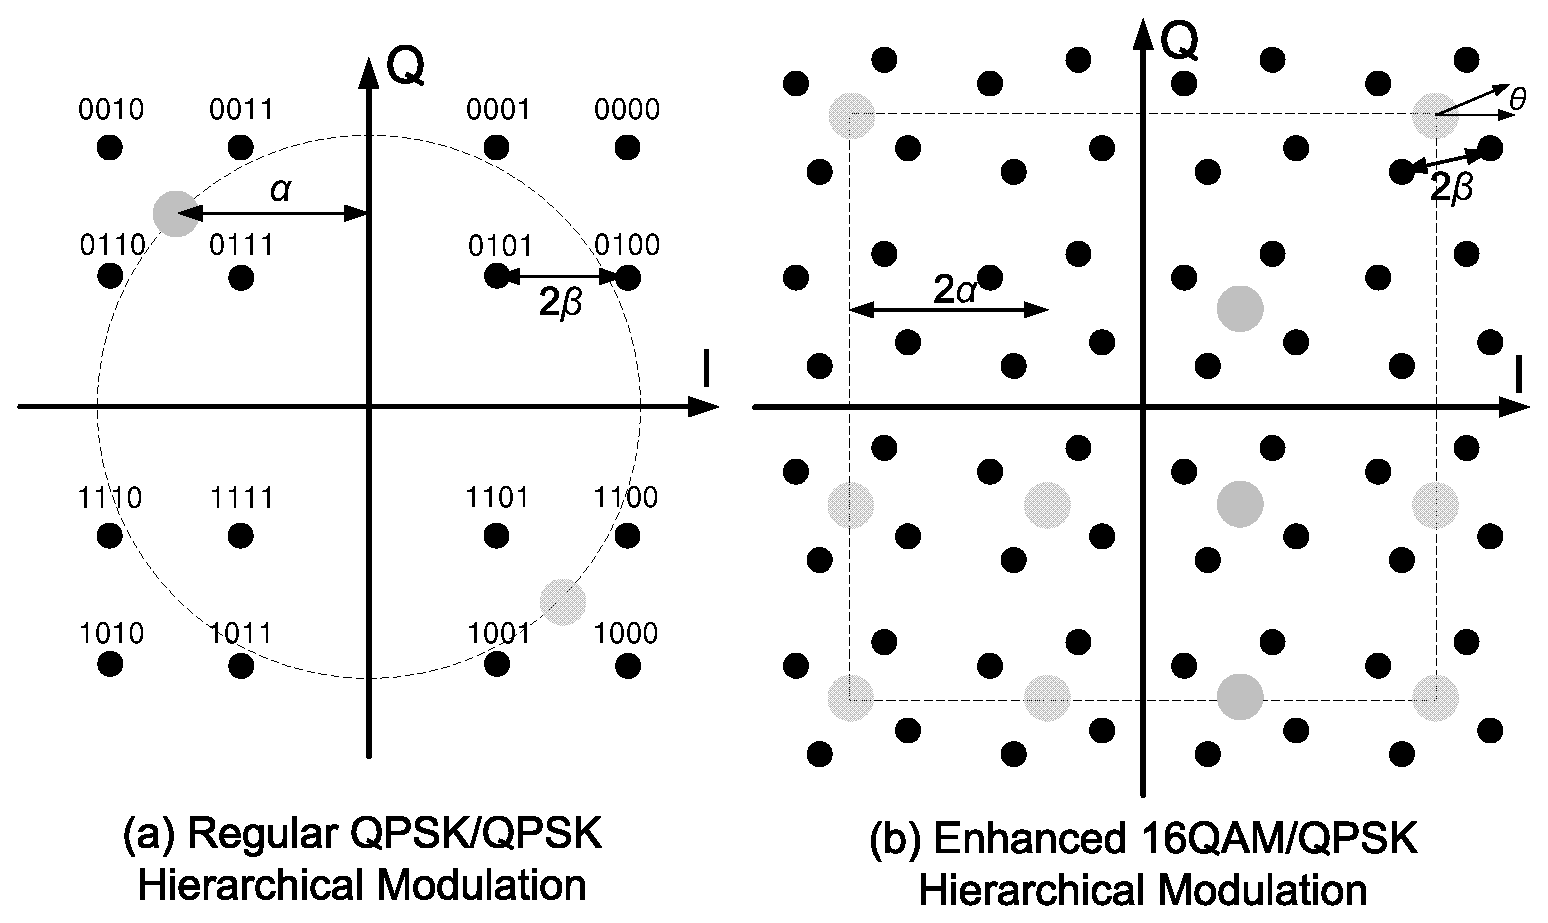
\includegraphics[width=3.50in, angle=0]{HierarchicalModulations.eps}
\caption{Regular and enhanced hierarchical modulations: the base
layer is QPSK/16QAM and the enhancement layer is
QPSK.}\label{regular_hierarchical} }
\end{figure}
\noindent Smaller MED usually results in more ambiguity and more
demodulation errors especially when $\zeta$ is large. The power
ratio or energy ratio $\zeta$ between the base layer and
enhancement layer is defined by
\begin{equation}
\begin{array}{rcl}
\zeta & = & \frac{P_{\mbox{\tiny B}}}{P_{\mbox{\tiny E}}}
\end{array}\label{power_ratio}
\end{equation}
\noindent with the default $\zeta > 1$. For QPSK/QPSK hierarchical
modulation, the power-splitting ratio is $\zeta_{\mbox{\tiny
QPSK/QPSK}}= \frac{\alpha^{2}}{\beta^{2}}$. For 16QAM/QPSK
modulation, $\zeta_{\mbox{\tiny 16QAM/QPSK}}=
\frac{4\alpha^{2}}{\beta^{2}}$. When $\zeta_{\mbox{\tiny
QPSK/QPSK}}=4$, the QPSK/QPSK modulation in
Fig.~\ref{regular_hierarchical}(a) becomes regular square-shaped
16QAM. In general, the enhancement-layer signal can be taken as
additional noise to the base layer. Therefore most existing
conventional receivers may continue to demodulate base-layer
signals with no additional change but at a lower
signal-to-noise-and-interference ratio (SINR) $\hat{\gamma}$
defined by
\begin{equation}
\begin{array}{rcccccl}
\hat{\gamma}& = & \frac{P_{\mbox{\tiny B}}}{P_{\mbox{\tiny
E}}+\sigma_{n}^{2}}&<&\gamma&=&\frac{P_{\mbox{\tiny
B}}}{\sigma_{n}^{2}}
\end{array}\label{SINR}
\end{equation}
\noindent with the background additive Gaussian white noise (AWGN)
power $\sigma_{n}^{2}$.

Regular hierarchical modulation may seriously suffer from ILI,
which not only decreases the base-layer SINR from ${\gamma}$ to
$\hat{\gamma}$ but also lowers the achievable spectral efficiency.
In order to minimize ILI, we proposed to optimize the signal
constellation with optimally rotating the enhancement-layer signal
sub-constellation. For the QPSK/QPSK hierarchical modulation shown
in Fig.~\ref{regular_hierarchical}(a), the QPSK signal
constellation of the enhancement layer is rotated in
counter-clockwise by $\theta\in\left[0\ \frac{1}{4}\pi\right]$.
The question now becomes how to choose the parameter $\theta$ for
each modulation. In the following, four schemes are proposed from
different perspectives of signal modulation and demodulation.

\section{Optimizing Hierarchical Modulation}
\subsection{Maximizing Achievable Rates~\label{Info_Theory}}
In general, the achievable rate of a $N$-ary modulated signal, of
either regular or hierarchical signal constellation, through AWGN
channel is given by~\cite{Unge82}
\begin{equation}
\begin{array}{lcl}
R&=&\log_{2}\left(N\right)-\\
&&\hspace{-0.20in}\frac{1}{N}\sum\limits_{i=0}^{N-1}\mbox{E}\left\{\log_{2}\left[\sum\limits_{j=0}^{N-1}e^{-\frac{\left|s_{j}+n-s_{i}\right|^2-\left|n\right|^2}{2\sigma^2}}\right]\right\}\
.
\end{array}\label{N_ary}
\end{equation}
\noindent This is the achievable rate when a receiver tries to
decode the whole hierarchically modulated symbol. Though the rate
in (\ref{N_ary}) is achievable for a user capable to decode the
whole constellation, it is more than achievable for a user with a
conventional receiver and detecting the base-layer signals only.
The achievable rate of either base layer or enhancement layer
along is lower than the total rate in (\ref{N_ary}). Following the
concept of the successive interference cancellation, the
achievable rate, also termed {\em equivalent capacity}, for a
receiver decoding up to $l$ layers of a hierarchical modulated
symbol is~\cite{Huber94}
\begin{equation}
\begin{array}{rcccl}
\tilde{R}_{l}&=&\sum\limits_{i=0}^{l-1}R_{i}& = &
R-\sum\limits_{j=l}^{L}{R}_{j}
\end{array}.\label{R_equiv}
\end{equation}

For the hierarchical modulation is 16QAM/QPSK-modulated with the
16QAM-modulated base layer, the achievable equivalent capacities
of each layer are shown in Fig.~\ref{capacity_rotating}, where the
total SNR fixed at $\frac{P}{\sigma^2}=20\mbox{dB}$ and the power
of the 16QAM sublayer changing from $50\%$ to $100\%$ of the total
power $P$. One of the interesting things shown is the equivalent
capacity of the 16QAM base layer changes periodically instead of
monotonically with increase the power ratio of the base layer.
However, this kind of capacity loss can be recovered by optimally
rotating the enhancement layer. This is one of the advantages of
the proposed enhanced hierarchical modulations.
\begin{figure}
\center{
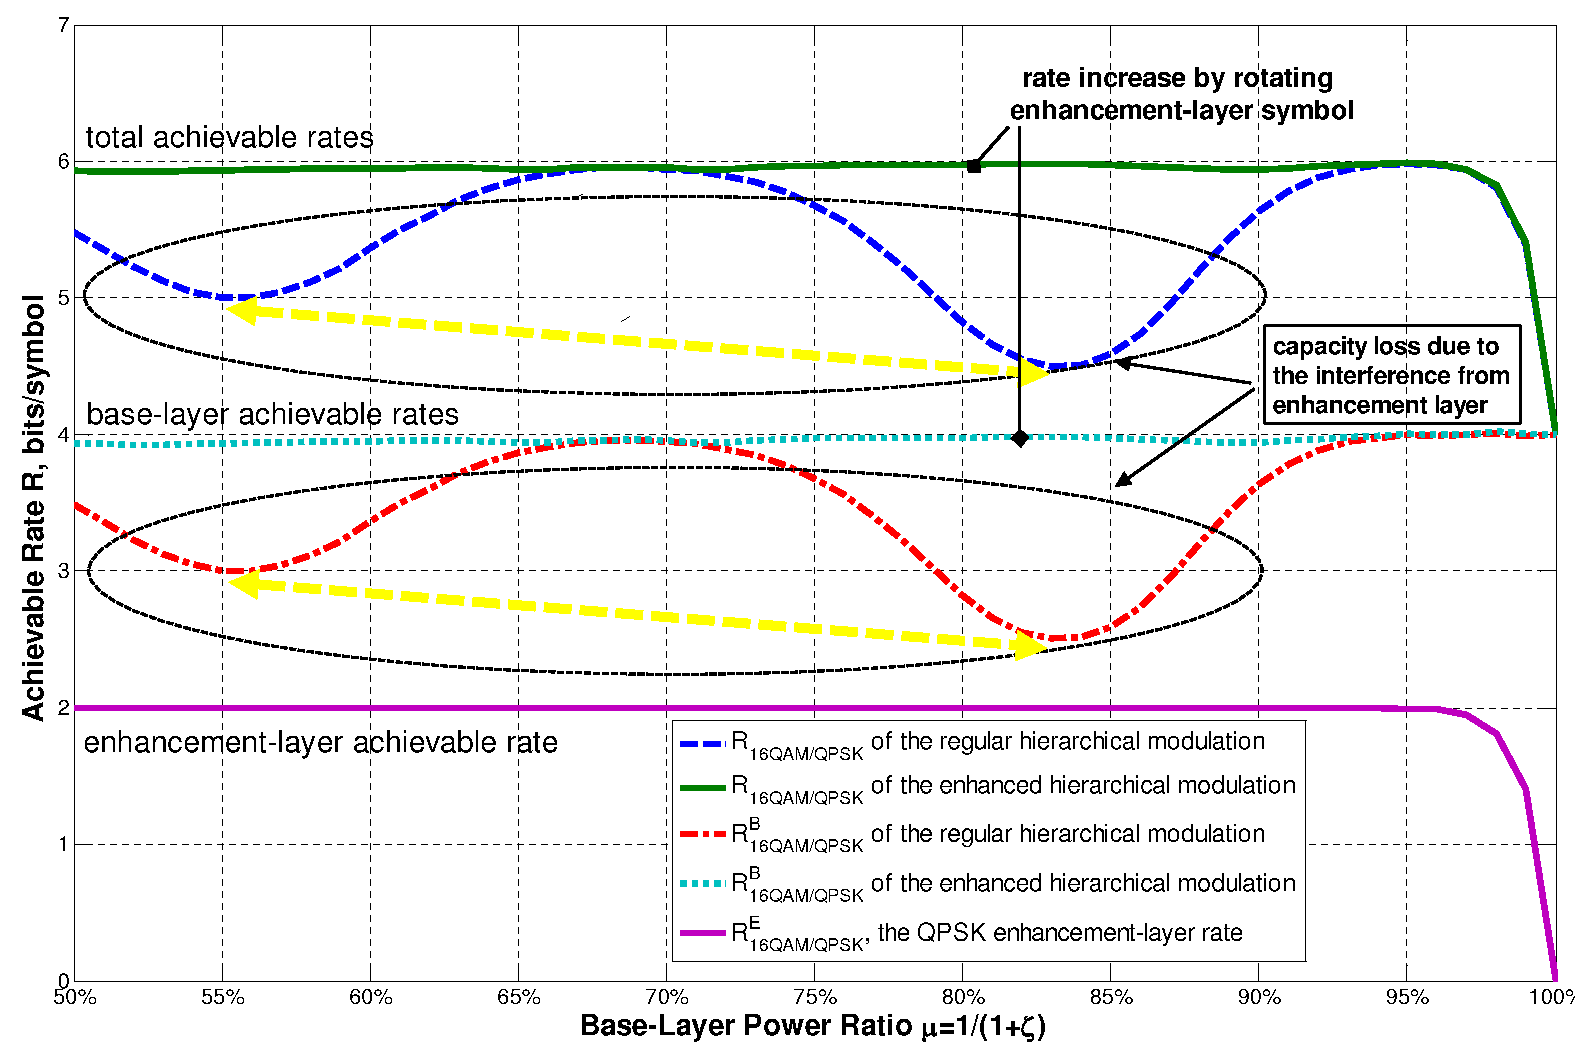
\includegraphics[width=3.50in, angle=0]{Capacity_power_splitting.eps}
\caption{Achievable rates of 16QAM/QPSK hierarchical modulation
with different power splitting and
$\frac{P}{\sigma^2}=20$dB.}\label{capacity_rotating} }
\end{figure}

\subsection{Maximizing Modulation Efficiency}
\begin{figure} \center{
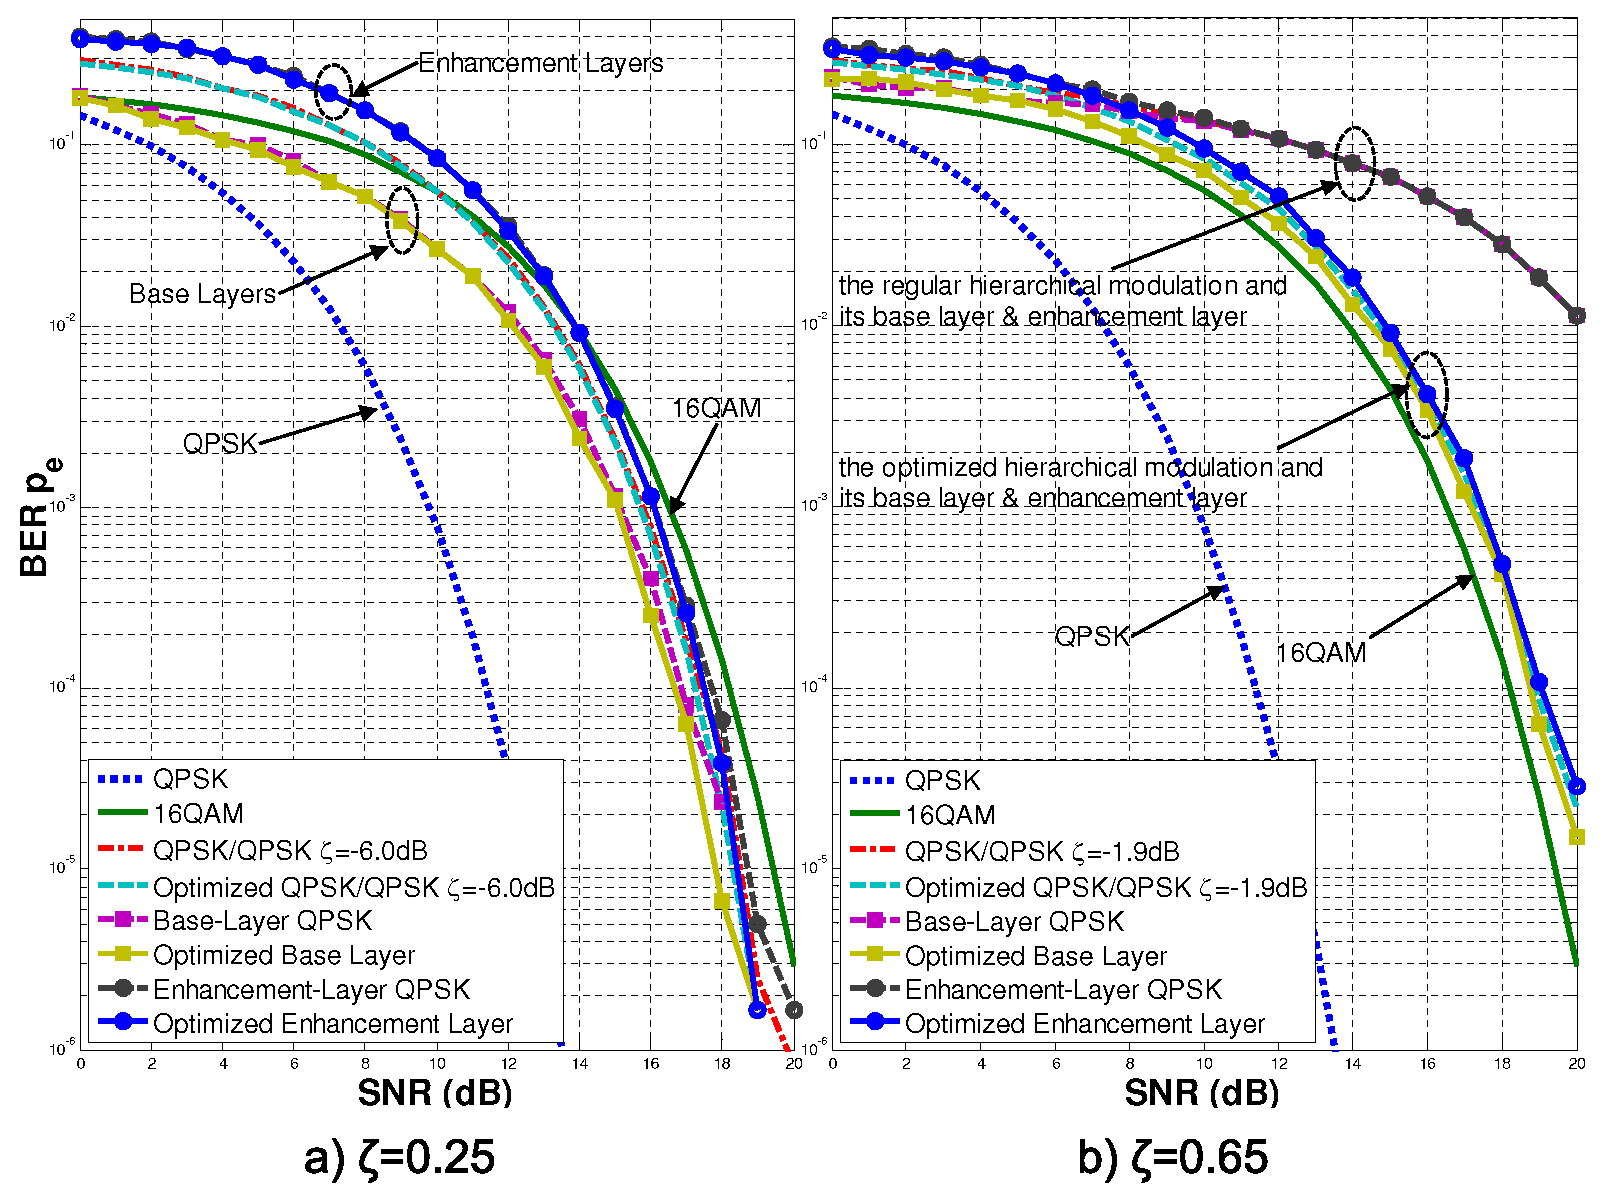
\includegraphics[width=3.50in, angle=0]{BER_Hierarchical.eps}
\caption{Bit-error rate of uncoded QPSK/QPSK hierarchical
modulations using maximum likelihood demodulation . } \label{BER}}
\end{figure}

From a signal processing standpoint, demodulation error and
capacity degradation may happen when there is unknown interference
or a change of interference distribution, even though the received
SNR $\gamma$ is the same. The BER performance of regular QPSK/QPSK
becomes deteriorated in Fig. \ref{BER} when $\zeta_{\mbox{\tiny
QPSK/QPSK}}$ increases. However, with optimally rotating the
enhancement-layer signal constellation, the performance loss can
be recovered. This kind of recovery is more significant with large
$\zeta$. In order to quantify and understand this kind of BER
performance loss due to interference and receiver design, one
approach we propose for capturing this kind of degradation is to
calculate the effective signal-to-noise ratio (ESNR) of the whole
transceiver chain, which is defined by
\begin{equation}
\begin{array}{rcl}
\tilde{\gamma}\left(\gamma\right)&\equiv&\Psi^{-1}\left({\rm
P}_{e}\left(\gamma\right)\right)
\end{array},\label{eff_SNR}
\end{equation}
\noindent where ${\rm P}_{e}(\gamma)$ is the demodulation BER of
the signal with SNR $\gamma$, and $\Psi^{-1}\left(\ast\right)$
denotes the inverse function of $\Psi\left(\cdot\right)$, the
demodulation error probability function with no ILI. The ESNR for
the QPSK-modulated base layer or enhancement layer of any
hierarchical modulation can be calculated by
\begin{equation}
\begin{array}{rcl}
\tilde{\gamma}_{\mbox{\tiny QPSK/QPSK}}&=&2\left[{\rm
Q}^{-1}\left({\rm P}_{e}\left(\gamma\right)\right)\right]^2
\end{array}.\label{eff_SNR_QPSK}
\end{equation}
\noindent More specifically, the ESNR for the base layer of
regular QPSK/QPSK hierarchical modulation with ML demodulator is
given by
\begin{equation}\hspace{-0.00in}
\begin{array}{l}
\tilde{\gamma}_{\mbox{\tiny QPSK/QPSK}}^{\mbox{\tiny
B}}(\gamma)=2\left[{\rm Q}^{-1}\left(\frac{{\rm
Q}\left((\sqrt{\zeta}+1)\sqrt{\frac{\gamma}{2\zeta+2}}\right)+{\rm
Q}\left((\sqrt{\zeta}-1)\sqrt{\frac{\gamma}{2\zeta+2}}\right)}{2}\right)\right]^2.
\end{array}\label{eff_SNR_QPSK_QPSK}
\end{equation}

By normalizing ESNR with $\gamma$, we can obtain hierarchical
modulation efficiency (ME) $\eta$ by
\begin{equation}
\begin{array}{rcccl}
\eta\left(\gamma\right)&=&\frac{\tilde{\gamma}}{\gamma}&=&\frac{1}{\gamma}\Psi^{-1}\left({\rm
P}_{e}(\gamma)\right)
\end{array}.\label{mod_eff}
\end{equation}
\noindent With no interference, $\eta\left(\gamma\right)=1$;
otherwise, $\eta\left(\gamma\right)<1$. $\eta$ is also the measure
of inter-layer resistance for hierarchical modulation. The high ME
value means stronger interference-resistance the modulated signal
has. The ME of QPSK/QPSK hierarchical modulation are plotted in
Fig. \ref{modulation_efficiency}. We can see the enhanced
hierarchical modulation has higher ME than the regular modulation.
The difference is more obvious when $\zeta$ becomes large. This
means the enhanced hierarchical modulation has the stronger
inter-layer interference resistance than that of regular
hierarchical modulation.
\begin{figure}
\center{
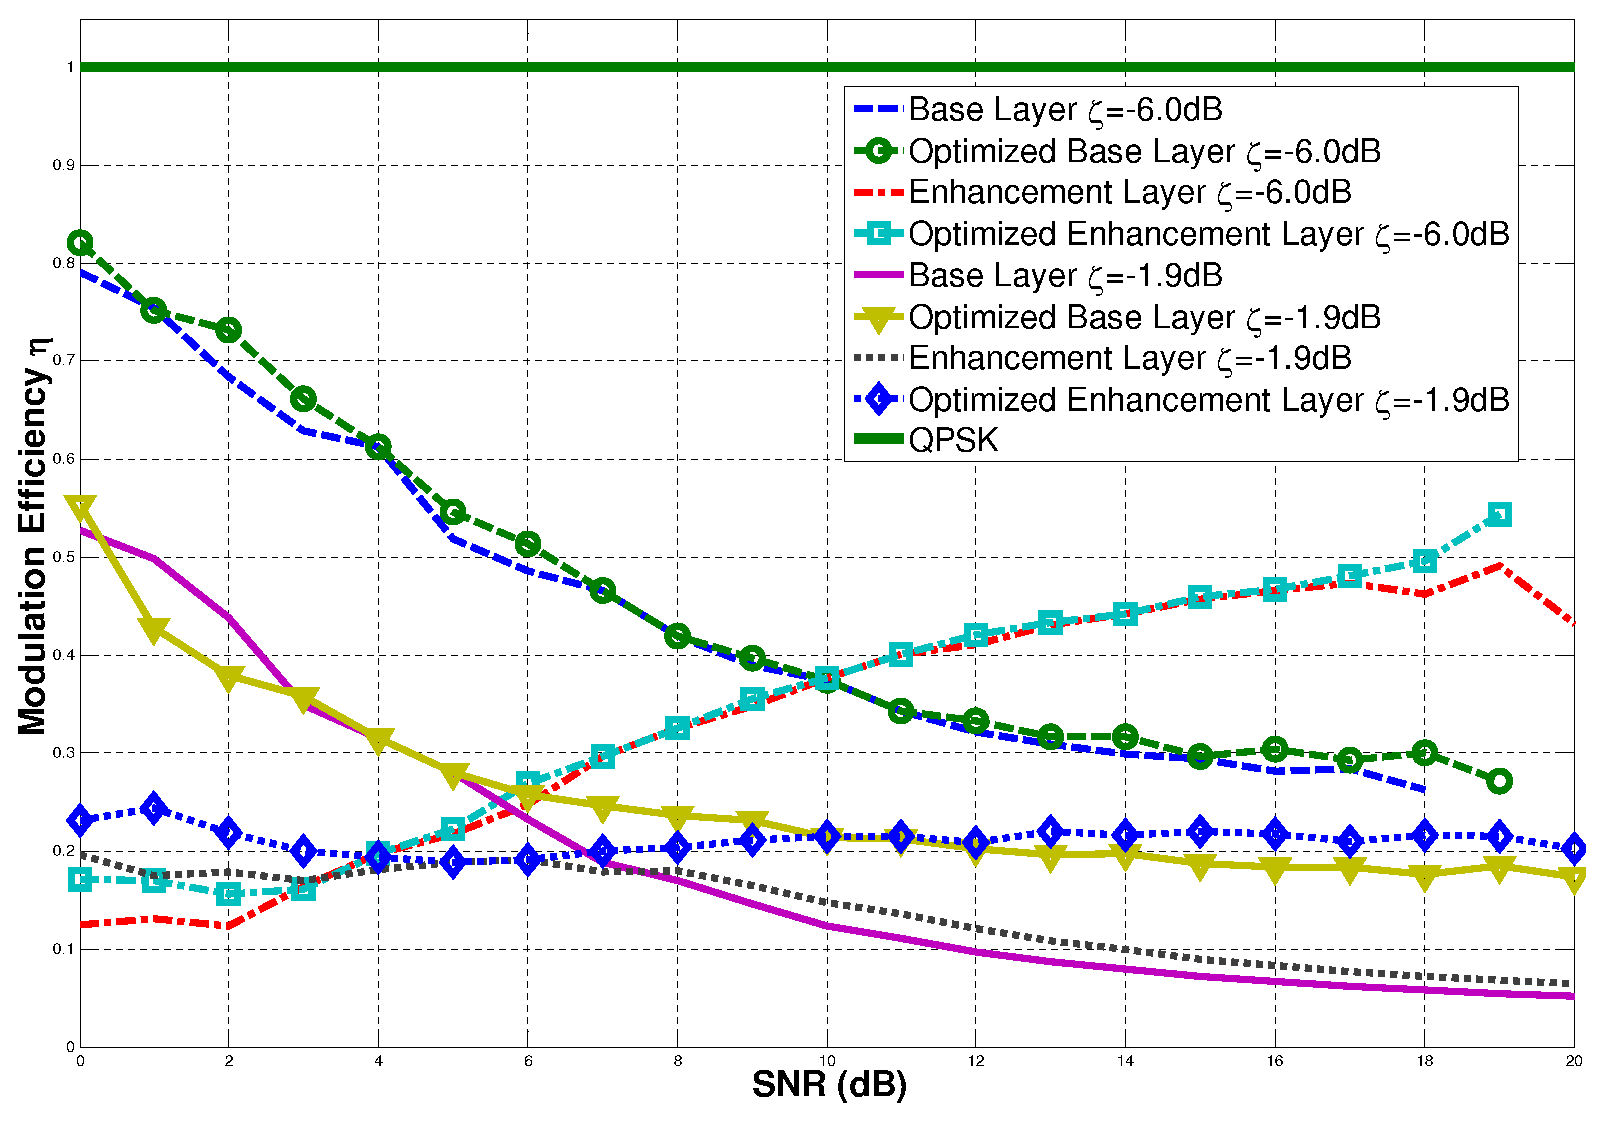
\includegraphics[width=3.50in, angle=0]{Modulation_Efficiency.eps}
\caption{Hierarchical modulation efficiency of QPSK/QPSK
hierarchical modulation using maximum likelihood
demodulation.}\label{modulation_efficiency} }
\end{figure}

Furthermore, in order to isolate the noise effect from
demodulation/decoding, the asymptotic modulation efficiency (AME)
$\eta_{\infty}$ is given by
\begin{equation}
\begin{array}{rcccl}
\eta_{\infty}&=&\lim\limits_{\gamma\rightarrow\infty}\eta\left(\gamma\right)&=&\lim\limits_{\sigma\rightarrow0}\frac{\sigma^2}{P}\Psi^{-1}\left(p_{e}\right)
\end{array},\label{asy_mod_eff}
\end{equation}
\noindent which is the ME in high SNR region. For the ME in
(\ref{eff_SNR_QPSK_QPSK}), the AME can be calculated by
\begin{equation}%\hspace{-0.10in}
\begin{array}{rcl}
\eta_{\infty}&=&\\
&&\hspace{-0.80in}\lim\limits_{\gamma\rightarrow\infty}\frac{2}{\gamma}\left[{\rm
Q}^{-1}\left(\frac{{\rm
Q}\left((\sqrt{\zeta}+1)\sqrt{\frac{\gamma}{2\zeta+2}}\right)+{\rm
Q}\left((\sqrt{\zeta}-1)\sqrt{\frac{\gamma}{2\zeta+2}}\right)}{2}\right)\right]^2.
\end{array}\label{asy_eff_SNR_QPSK_QPSK}
\end{equation}
\noindent With (\ref{asy_mod_eff}) and
(\ref{asy_eff_SNR_QPSK_QPSK}), it shows that AME indicates how
fast ESNR is approaching SNR when $\gamma\rightarrow\infty$. This
can be expressed by
\begin{equation}
\begin{array}{rcl}
\eta_{\infty}&=&\frac{\partial\eta\left(\gamma\right)}{\partial\gamma}|_{\gamma=\infty}
\end{array}.\label{asy_mod_eff2}
\end{equation}
\noindent The AME for QPSK/QPSK hierarchical modulation can also
be found in Fig.~\ref{modulation_efficiency}, where they are the
points when SNR becomes larger and larger. The AME of a
hierarchical modulation only depends on its signal constellation
design and is independent to the background noise.

\subsection{Maximizing Demodulation Robustness}
In pilot-assisted transmission (PAT), pilot symbols are
periodically inserted into the data symbols for assisting the
receiver to estimate the channel fading. An overview of PAT
including the pilot placement and channel estimation can be found
in~\cite{Tong04}. In the receiver side, after matched filtering
and sampling with perfect symbol timing at the rate of $1/T_{s}$,
a baseband $T_s$-spaced discrete-time complex-valued signal can be
represented by
\begin{equation}
\begin{array}{rcl}
r_{k}&=&h_{k}s_{k}+n_{k}
\end{array}.
\end{equation}
\noindent The sequence $s_{k}$ represents complex modulated
symbols. The sequence $h_{k}$ represents the channel. For Rayleigh
channels, it is a complex zero-mean Gaussian random variable, and
$n_{k}$ is AWGN with variance $\sigma_{n}^2$. At the receiver, the
channel fading $h_{k}$ is extracted and interpolated to be
$\hat{h}_{k}$ with the help of known pilot symbols. If a minimum
mean squared error (MMSE) equalizer is applied, the output can be
written by

\begin{equation}\hspace{-0.05in}
\begin{array}{rcccl}
\hat{s}_{k}&=&\frac{\hat{h}^{\ast}_{k}}{\hat{h}_{k}\hat{h}_{k}^{\ast}+\sigma_{n}^{2}}r_{k}
&=&\frac{h_{k}\hat{h}^{\ast}_{k}}{\hat{h}_{k}\hat{h}_{k}^{\ast}+\sigma_{n}^{2}}s_{k}+\frac{\hat{h}^{\ast}_{k}}{\hat{h}_{k}\hat{h}_{k}^{\ast}+\sigma_{n}^{2}}n_{k}
\end{array}\label{MMSE_eq}
\end{equation}

\noindent When the SNR of received signals is high,
(\ref{MMSE_eq}) can be simplified by

\begin{equation}
\begin{array}{rcl}
\hat{s}_{k}&=&\frac{h_{k}}{\hat{h}_{k}}s_{k}+\frac{h_{k}}{\hat{h}_{k}}n_{k}
\end{array}\label{MF_eq}
\end{equation}

\noindent which essentially becomes a match-filter equalizer. For
a regular QPSK/QPSK hierarchical modulation, the base-layer
symbols are demodulated by comparing the received signal withe the
zero-point of I and Q channels. This means the QPSK demodulation
is independent to the channel amplitude estimation error. However,
if there is channel phase estimation error $\phi$, the resulted
signal will be improperly rotated. With (\ref{BER_QPSK}), the
uncoded BER of base-layer QPSK demodulations is

\begin{equation}\hspace{-0.15in}
\begin{array}{rcl}
{\rm P}_{e,\mbox{\tiny QPSK/QPSK}}^{\mbox{\tiny B}}\left(\gamma,\ \zeta\right)&=&\frac{1}{2}Q\left(\left(\sqrt{\zeta}+1\right)\sqrt{\frac{\gamma}{2(\zeta+1)}}\cos\phi\right)\\
&&\hspace{-0.10in}+\frac{1}{2}Q\left(\left(\sqrt{\zeta}-1\right)\sqrt{\frac{\gamma}{2(\zeta+1)}}\cos\phi\right)
\end{array}\label{BL_BER}
\end{equation}

\noindent If the enhancement-layer signal constellation is rotated
by $\theta$, the resulted uncoded BER becomes

\begin{equation}%\hspace{-0.0in}
\begin{array}{rcl}
%{\rm P}_{e,\mbox{\tiny QPSK}}^{\mbox{\tiny B}}\left(A_{\mbox{\tiny B}}, A_{\mbox{\tiny E}},\ \theta\right)&=&\frac{1}{4}Q\left(\left[A_{\mbox{\tiny B}}+\sqrt{2}\cos(\theta+\frac{1}{4}\pi)A_{\mbox{\tiny E}}\right]\frac{h\cos\phi}{\sigma_{n}}\right)\\
{\rm P}_{e,\mbox{\tiny QPSK/QPSK}}^{\mbox{\tiny B}}\left(\gamma,\ \zeta,\ \theta\right)&=&\\
&&\hspace{-1.4in}\frac{1}{4}\sum\limits_{i=1}^{4}Q\left(\left[\sqrt{\zeta}+\sqrt{2}\cos(\theta+\frac{i}{4}\pi)\right]\sqrt{\frac{\gamma}{2(\zeta+1)}}\cos\phi\right)
%&&\hspace{-1.2in}\frac{1}{4}Q\left(\left[\sqrt{\zeta}+\sqrt{2}\cos(\theta+\frac{1}{4}\pi)\right]\sqrt{\frac{\gamma}{2(\zeta+1)}}\cos\phi\right)\\
%&&\hspace{-1.3in}+\frac{1}{4}Q\left(\left[\sqrt{\zeta}+\sqrt{2}\cos(\theta+\frac{3}{4}\pi)\right]\sqrt{\frac{\gamma}{2(\zeta+1)}}\cos\phi\right)\\
%&&\hspace{-1.3in}+\frac{1}{4}Q\left(\left[\sqrt{\zeta}+\sqrt{2}\cos(\theta+\frac{5}{4}\pi)\right]\sqrt{\frac{\gamma}{2(\zeta+1)}}\cos\phi\right)\\
%&&\hspace{-1.3in}+\frac{1}{4}Q\left(\left[\sqrt{\zeta}+\sqrt{2}\cos(\theta+\frac{7}{4}\pi)\right]\sqrt{\frac{\gamma}{2(\zeta+1)}}\cos\phi\right)
\end{array}.\label{BL_BER_rotated}
\end{equation}

\noindent With properly choosing the rotation angle $\theta$, the
enhanced hierarchical modulation may help reduce the demodulation
error rate at the receiver side. This can be shown in
Fig.~\ref{amplitude_error} and \ref{phase_error}.

\begin{figure} \center{
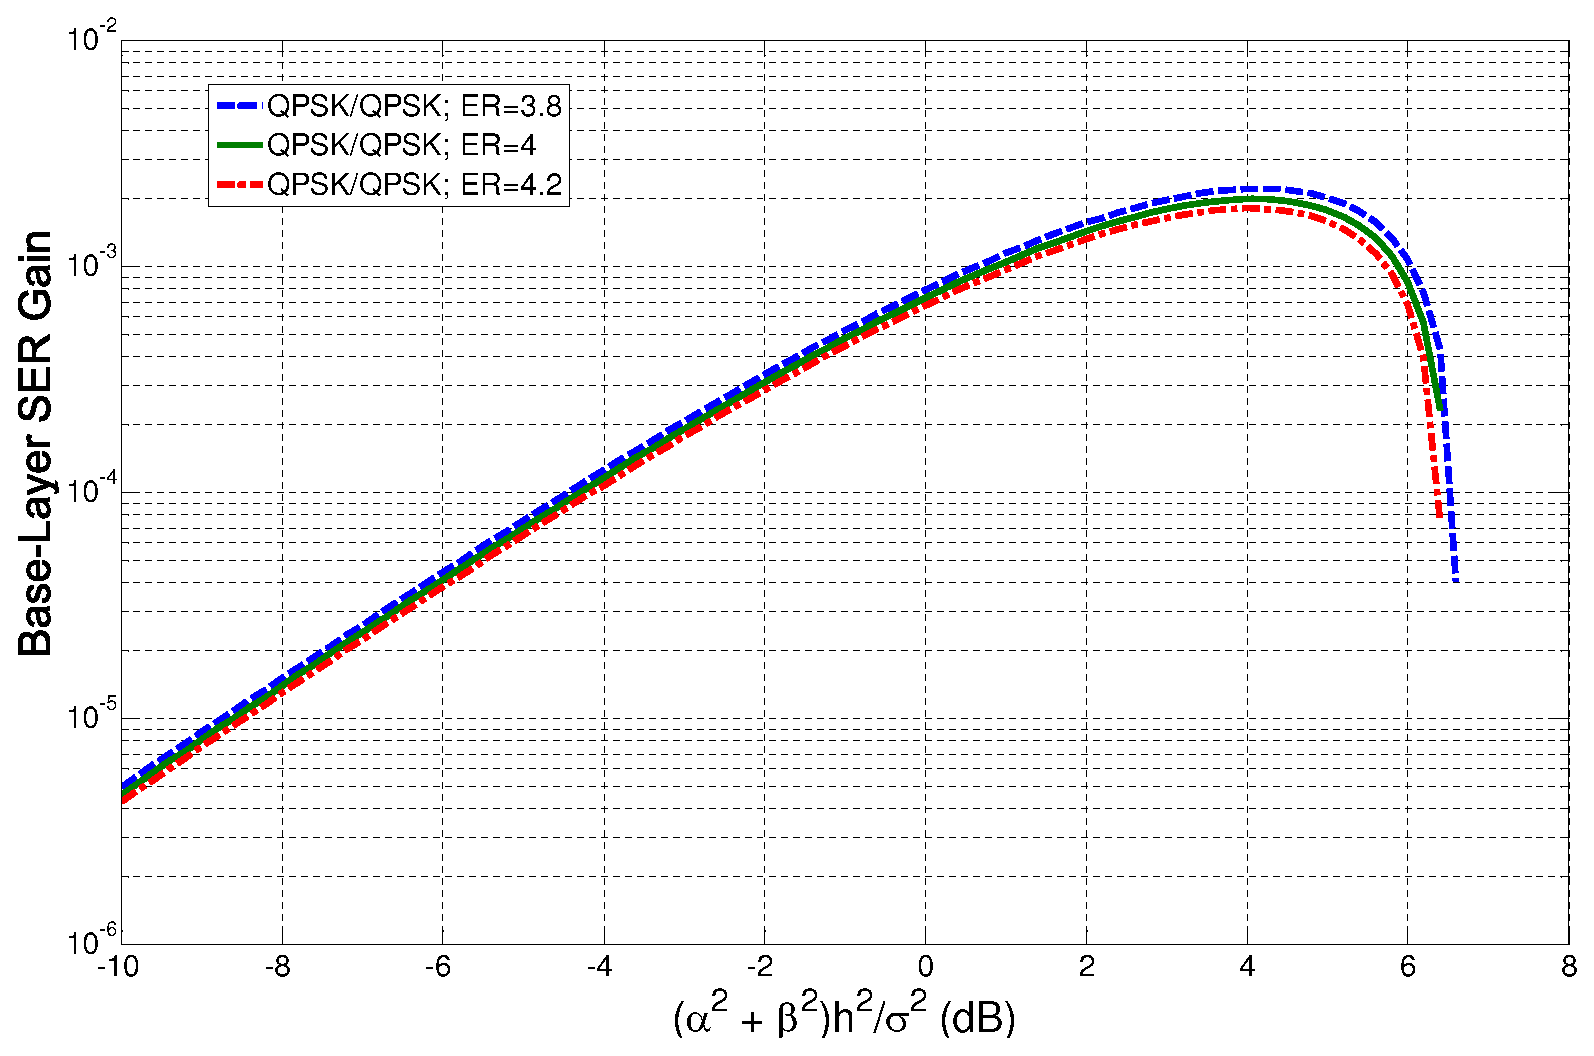
\includegraphics[width=3.50in, angle=0]{Robust_Amplitude.eps}
\caption{The base-layer SER gain with optimally rotating
enhancement-layer symbols. }\label{amplitude_error}}
\end{figure}

\begin{figure} \center{
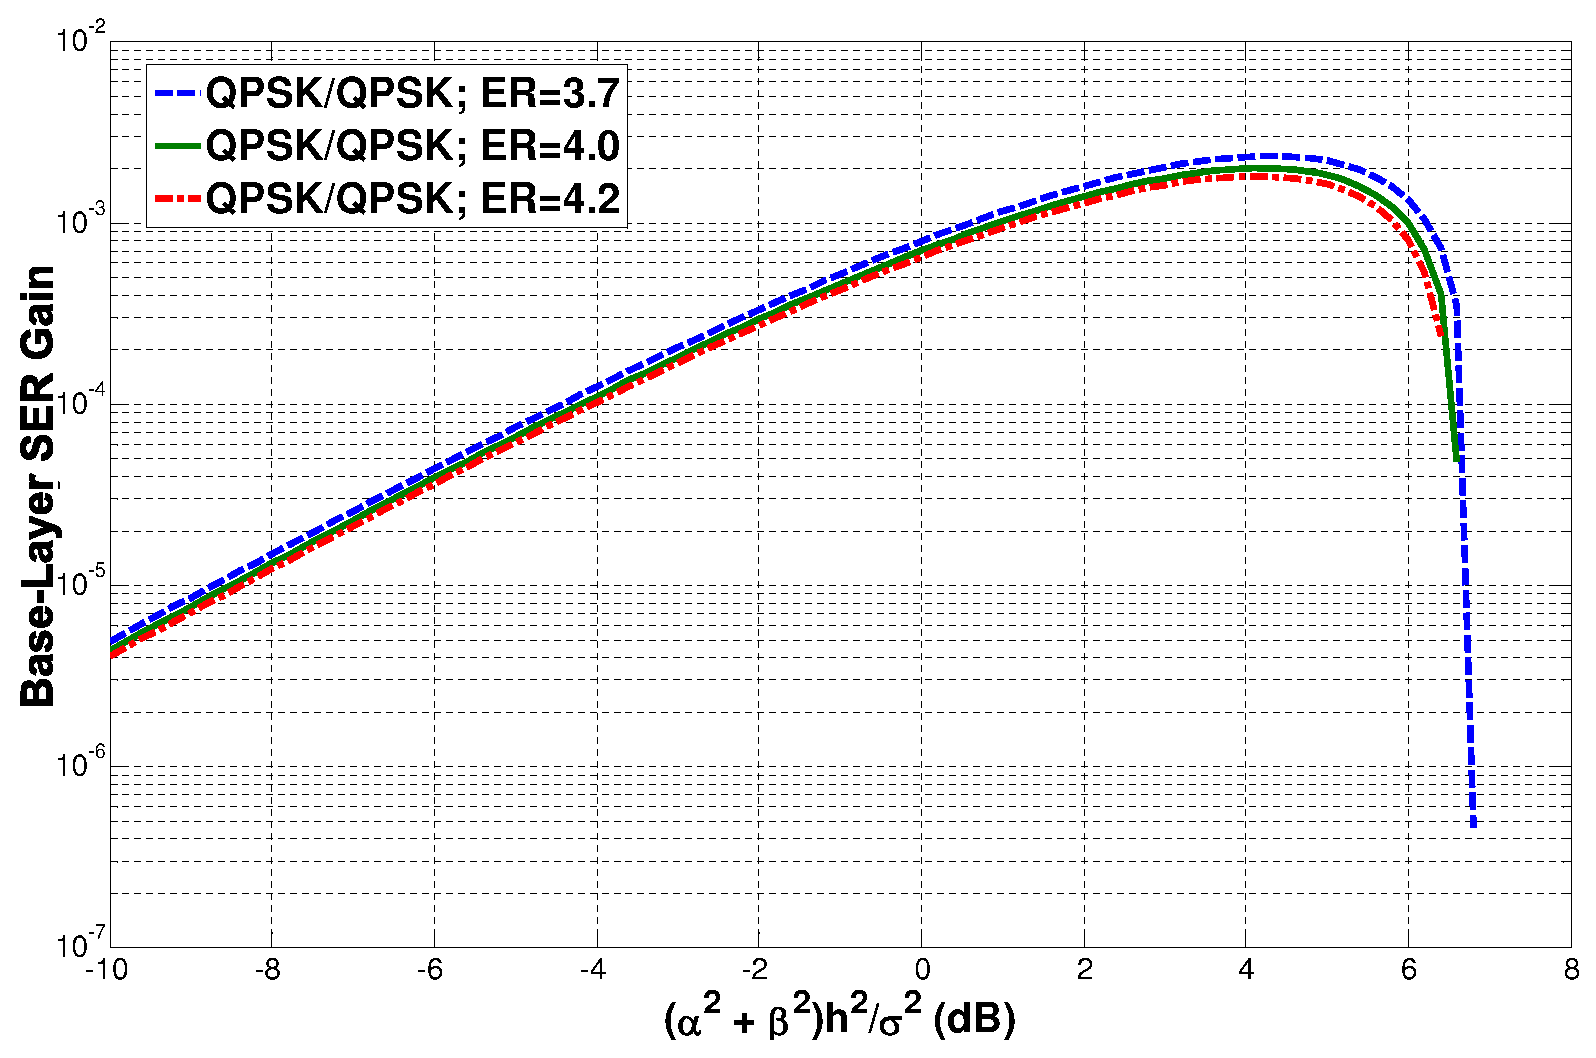
\includegraphics[width=3.50in, angle=0]{Robust_Phase.eps}
\caption{The base-layer SER gain with optimally rotating
enhancement-layer symbols and the channel phase estimation error
$\phi=10^o$. }\label{phase_error}}
\end{figure}

\subsection{Minimizing Peak-to-Average-Power Ratio}
Since OFDM has been widely adopted and intensively studied for
next-generation wireless systems, it is important to understand
how the enhanced hierarchical modulation works with OFDM. Here we
investigated the PAPR reduction performance when it is transmitted
over OFDM. An OFDM signal is the sum of $L$ independent modulated
symbols $\left\{s_{l}:\ 1\leq l\leq L\right\}$ mapped onto $L$
different subcarriers with the frequency separation $\frac{1}{T}$,
where $T$ is the symbol period with no additional overhead such as
cyclic prefix (CP) and zero prefix (ZP). At the transmitter side,
the discrete time-domain samples $\left\{x_{m}:\ 1\leq m\leq
L\right\}$ are the inverse fast Fourier transform (IFFT) of the
complex symbols $\left\{s_{l}:\ 1\leq l\leq L\right\}$:
\begin{equation}
\begin{array}{lcl}
x_{m}&=&\frac{1}{\sqrt{L}}\sum\limits_{l=0}^{L-1}s_{l}e^{j2\pi\frac{ml}{L}}
\end{array}.\label{OFDM}
\end{equation}
\noindent Before transmission, $x_{m}$ is usually extended by
attaching a CP or ZP. When CP is applied, the extended OFDM symbol
\begin{equation}
\begin{array}{rcl}
\tilde{x}_{n}&=&\Bigg\{ \begin{array}{ll}x_{n}&1\leq n\leq L\\
x_{n+L}&-L_{cp}+1\leq n\leq 0 \end{array}
\end{array}.
\end{equation}
\noindent The extended OFDM symbol then passes through
digital-to-analog converter and pulse-shaping filter before
up-converted to the carrier frequency. The PAPR of OFDM signal is
usually defined by
\begin{equation}
\begin{array}{rcl}
\xi&=&\frac{1 }{\mbox{E}\left\{\left|x_{m}\right|^2\right\}
}\max\limits_{m} \left|x_{m}\right|^{2}
\end{array},
\end{equation}
\noindent though in practice the PAPR of the analog signal
equivalent of $\left\{\tilde{x}_{n}:\ -L_{cp}+1\leq n\leq
L\right\}$ is more of interest.

The PAPR values of the regular QPSK/QPSK hierarchical modulation
and its enhancement are plotted in Fig.~\ref{HM_PAPR}. It shows
that the PAPR of regular hierarchical modulation can be reduced
with optimally rotating enhancement-layer symbols. And when the
power splitting ratio $\eta$ becomes larger and larger, the PAPR
reduction performance will be more significant.
\begin{figure} \center{
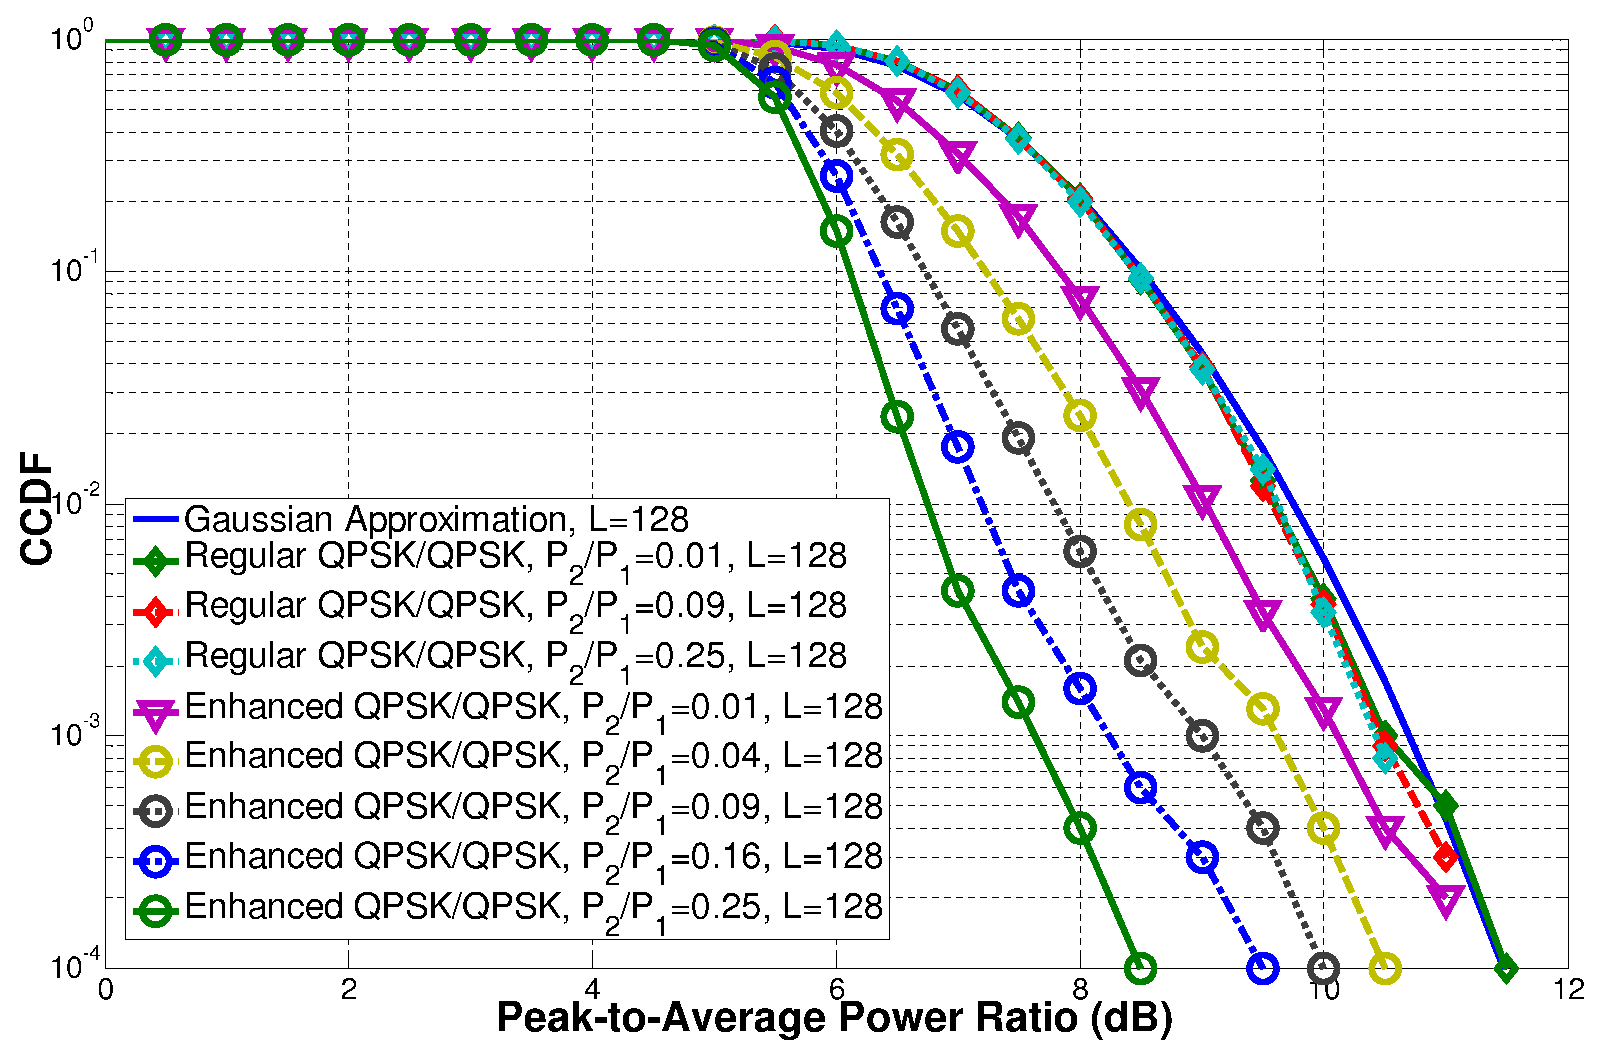
\includegraphics[width=3.50in, angle=0]{HM_PAPR.eps}
\caption{PAPRs of hierarchical modulations over OFDM with $L=128$.
} \label{HM_PAPR}}
\end{figure}


\section{Conclusions}
In this paper, one enhanced hierarchical modulation scheme and
four optimization approaches are proposed for higher throughput,
less error rate, more robustness and higher power efficiency. One
approach is to maximize the spectral efficiency, one approach is
to maximize modulation efficiency, another approach is to increase
the resistance to channel estimation errors and the last one is to
minimize the PAPR when it is used with OFDM. The rationales as
well as the performance of the proposed approaches are analyzed.
They can be used for helping upgrade and design BCMCS systems with
minimum complexity increase. It is adopted in the 3.5G standard
UMB by 3GPP2. \small
\bibliographystyle{unsrt}
\bibliography{Hierarchical_Modulation}
\end{document}
